%This section talks about that which is retelling in video games
\section{Retelling games}
% Re-Tellings: The Fourth Layer of Narrative as an Instrument for Critique - Mirjam Palosaari Eladhari
% When the Fourth Layer Meets the Fourth Wall: The Case for Critical Game Retellings - Steven Sych

%This section showcases examples of retelling in video games
\subsection{Examples of TTRPG retellings}
%Adventure Zone (Comic) & Critical Role (Cartoon)

%This section showcases examples 1of AI based retelling/storytelling
\subsection{Artificial Intelligence as a Reteller/storyteller}
%AI Comic factory and The Finals commentator

%In this section we will look at comic studies and use that as a basis for the project
\section{Comic books}
%Understanding Comics (Scott McCloud) and Comics and Sequential Art (Will Eisner)
Making Comic Books is an art form on its own and to understand how to generate a comic book with AI we need to understand how comic books function as an artefact: How they are made; How they are structured; How they are read; And what comic books are. This section will look at comic book studies to create a better understanding of comic book creation.

Comic books are a sequential art form\cite{eisner2008comics}. When you take a comic book panel and look at it outside of the context of other panels it is just an image. But when you place them side by side in a sequential order the pictures become a comic book \ref{fig:Sequential Art}. Looking at the image we can see that an image of a man holding its hat is just a man holding a hat. But when you place two images of a man holding his hat side by side we can see that it creates a motion of tipping his hat.

\begin{figure}[!htp]
	\centering
	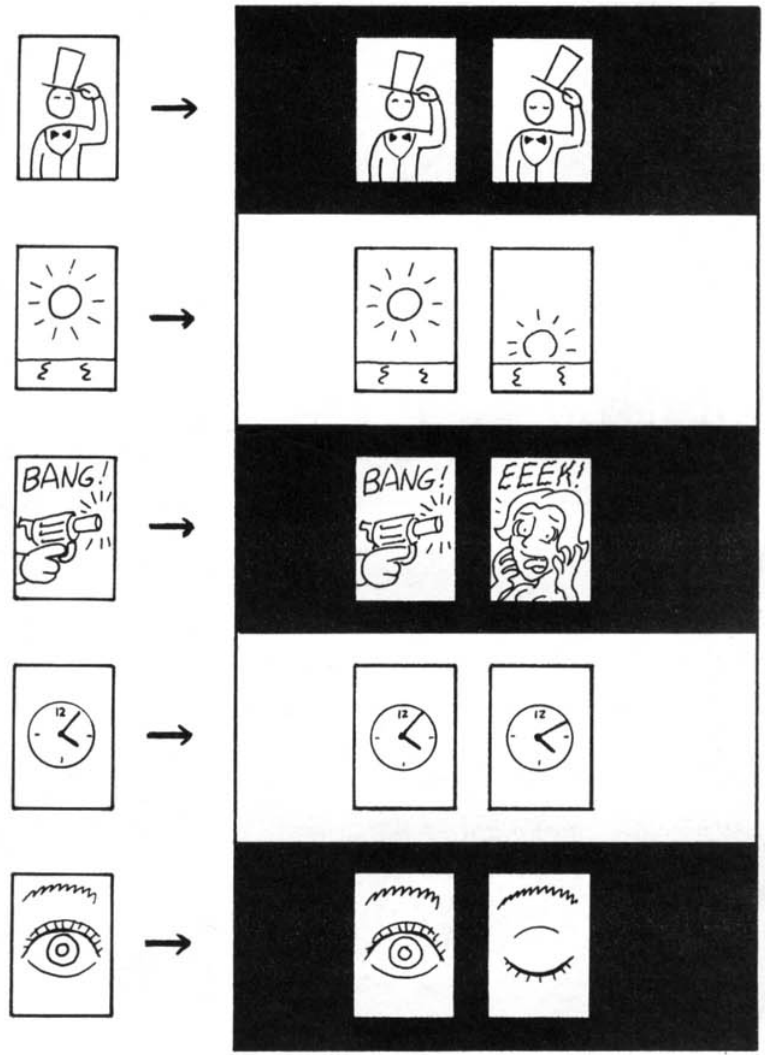
\includegraphics[scale=0.45]{images/SequentalArtUnderstandingComicPage5.png}
	\caption[Sequential Art]{Sequential Art (Understanding Comics Scott McCloud page 5)}
	\label{fig:Sequential Art}
\end{figure}



\subsection{Comic Book take aways}

%In this section we will look at the different AI models and why I chose them
\section{AI models}
There are many different AI models that floating around the internet that are open source and could be useful for this thesis. The make choose between all the available models a requirement list has been constructed based on the artifact requirements. In short the Speech recording model needs to transcribe audio recordings to text. The LLM model needs to be able to generate a comic book script based on the transcribed text. Including a prompt for the generative image model and the the text that needs to be placed on the comic panels.
The requirements:
LLM
Image generation
Speech recognition
%Talk about Stable Diffusion, Llama 3.1-8B and Whisper and why I chose them. Also talk about other models and why I did not choose them.

%In this section I will talk about the ethical consideration around AI usage.
\section{AI ethics}
%The Ethics of AI in games. – Melhart et al.
% Building ethics into artificial intelligence. – Yu et al.
% Deep Learning for Coders with Fastai and Pytorch: AI Applications Without a PhD – Jeremy Howard & Sylvain Gugger
% The ethics of Artificial Intelligence – Nick Bostrom & Eliezer Yudkowsky





